%%%%%%%%%%%%%%%%%%%%%%%%%%%%%%%%%%%%%%%%%%%%%%%%%%%%%%%%%%%%%%%%%%%%%%%%%%%%%%%%%%%%%%%%%%%%%%%%%%%%%%%%%%%%%%%%%%%%%%%%%%%%%%%%%%%%%%%%%%%%%%%%%%%%%%%%%%%
% This is just an example/guide for you to refer to when submitting manuscripts to Frontiers, it is not mandatory to use Frontiers .cls files nor frontiers.tex  %
% This will only generate the Manuscript, the final article will be typeset by Frontiers after acceptance.
%                                              %
%                                                                                                                                                         %
% When submitting your files, remember to upload this *tex file, the pdf generated with it, the *bib file (if bibliography is not within the *tex) and all the figures.
%%%%%%%%%%%%%%%%%%%%%%%%%%%%%%%%%%%%%%%%%%%%%%%%%%%%%%%%%%%%%%%%%%%%%%%%%%%%%%%%%%%%%%%%%%%%%%%%%%%%%%%%%%%%%%%%%%%%%%%%%%%%%%%%%%%%%%%%%%%%%%%%%%%%%%%%%%%

%%% Version 3.4 Generated 2018/06/15 %%%
%%% You will need to have the following packages installed: datetime, fmtcount, etoolbox, fcprefix, which are normally inlcuded in WinEdt. %%%
%%% In http://www.ctan.org/ you can find the packages and how to install them, if necessary. %%%

\documentclass[utf8]{frontiersSCNS}

%\setcitestyle{square} % for Physics and Applied Mathematics and Statistics articles
\usepackage{url,hyperref,lineno,microtype,subcaption}
\usepackage[onehalfspacing]{setspace}

\linenumbers


% BELOW TAKEN FROM rticles plos template
%
% amsmath package, useful for mathematical formulas
\usepackage{amsmath}
% amssymb package, useful for mathematical symbols
\usepackage{amssymb}

% hyperref package, useful for hyperlinks
\usepackage{hyperref}

% graphicx package, useful for including eps and pdf graphics
% include graphics with the command \includegraphics
\usepackage{graphicx}

% Sweave(-like)
\usepackage{fancyvrb}
\DefineVerbatimEnvironment{Sinput}{Verbatim}{fontshape=sl}
\DefineVerbatimEnvironment{Soutput}{Verbatim}{}
\DefineVerbatimEnvironment{Scode}{Verbatim}{fontshape=sl}
\newenvironment{Schunk}{}{}
\DefineVerbatimEnvironment{Code}{Verbatim}{}
\DefineVerbatimEnvironment{CodeInput}{Verbatim}{fontshape=sl}
\DefineVerbatimEnvironment{CodeOutput}{Verbatim}{}
\newenvironment{CodeChunk}{}{}

% cite package, to clean up citations in the main text. Do not remove.
\usepackage{cite}

\usepackage{color}

\providecommand{\tightlist}{%
  \setlength{\itemsep}{0pt}\setlength{\parskip}{0pt}}

% Below is from frontiers
%
\bibliographystyle{frontiersinSCNS}
% Use doublespacing - comment out for single spacing
%\usepackage{setspace}
%\doublespacing


% Leave a blank line between paragraphs instead of using \\


\def\keyFont{\fontsize{8}{11}\helveticabold }


%% ** EDIT HERE **
%% PLEASE INCLUDE ALL MACROS BELOW

%% END MACROS SECTION

% Pandoc citation processing

\usepackage{color}
\usepackage{fancyvrb}
\newcommand{\VerbBar}{|}
\newcommand{\VERB}{\Verb[commandchars=\\\{\}]}
\DefineVerbatimEnvironment{Highlighting}{Verbatim}{commandchars=\\\{\}}
% Add ',fontsize=\small' for more characters per line
\usepackage{framed}
\definecolor{shadecolor}{RGB}{248,248,248}
\newenvironment{Shaded}{\begin{snugshade}}{\end{snugshade}}
\newcommand{\AlertTok}[1]{\textcolor[rgb]{0.94,0.16,0.16}{#1}}
\newcommand{\AnnotationTok}[1]{\textcolor[rgb]{0.56,0.35,0.01}{\textbf{\textit{#1}}}}
\newcommand{\AttributeTok}[1]{\textcolor[rgb]{0.77,0.63,0.00}{#1}}
\newcommand{\BaseNTok}[1]{\textcolor[rgb]{0.00,0.00,0.81}{#1}}
\newcommand{\BuiltInTok}[1]{#1}
\newcommand{\CharTok}[1]{\textcolor[rgb]{0.31,0.60,0.02}{#1}}
\newcommand{\CommentTok}[1]{\textcolor[rgb]{0.56,0.35,0.01}{\textit{#1}}}
\newcommand{\CommentVarTok}[1]{\textcolor[rgb]{0.56,0.35,0.01}{\textbf{\textit{#1}}}}
\newcommand{\ConstantTok}[1]{\textcolor[rgb]{0.00,0.00,0.00}{#1}}
\newcommand{\ControlFlowTok}[1]{\textcolor[rgb]{0.13,0.29,0.53}{\textbf{#1}}}
\newcommand{\DataTypeTok}[1]{\textcolor[rgb]{0.13,0.29,0.53}{#1}}
\newcommand{\DecValTok}[1]{\textcolor[rgb]{0.00,0.00,0.81}{#1}}
\newcommand{\DocumentationTok}[1]{\textcolor[rgb]{0.56,0.35,0.01}{\textbf{\textit{#1}}}}
\newcommand{\ErrorTok}[1]{\textcolor[rgb]{0.64,0.00,0.00}{\textbf{#1}}}
\newcommand{\ExtensionTok}[1]{#1}
\newcommand{\FloatTok}[1]{\textcolor[rgb]{0.00,0.00,0.81}{#1}}
\newcommand{\FunctionTok}[1]{\textcolor[rgb]{0.00,0.00,0.00}{#1}}
\newcommand{\ImportTok}[1]{#1}
\newcommand{\InformationTok}[1]{\textcolor[rgb]{0.56,0.35,0.01}{\textbf{\textit{#1}}}}
\newcommand{\KeywordTok}[1]{\textcolor[rgb]{0.13,0.29,0.53}{\textbf{#1}}}
\newcommand{\NormalTok}[1]{#1}
\newcommand{\OperatorTok}[1]{\textcolor[rgb]{0.81,0.36,0.00}{\textbf{#1}}}
\newcommand{\OtherTok}[1]{\textcolor[rgb]{0.56,0.35,0.01}{#1}}
\newcommand{\PreprocessorTok}[1]{\textcolor[rgb]{0.56,0.35,0.01}{\textit{#1}}}
\newcommand{\RegionMarkerTok}[1]{#1}
\newcommand{\SpecialCharTok}[1]{\textcolor[rgb]{0.00,0.00,0.00}{#1}}
\newcommand{\SpecialStringTok}[1]{\textcolor[rgb]{0.31,0.60,0.02}{#1}}
\newcommand{\StringTok}[1]{\textcolor[rgb]{0.31,0.60,0.02}{#1}}
\newcommand{\VariableTok}[1]{\textcolor[rgb]{0.00,0.00,0.00}{#1}}
\newcommand{\VerbatimStringTok}[1]{\textcolor[rgb]{0.31,0.60,0.02}{#1}}
\newcommand{\WarningTok}[1]{\textcolor[rgb]{0.56,0.35,0.01}{\textbf{\textit{#1}}}}

\def\Authors{
  Chaochen Wang\,\textsuperscript{1},
  Suzana Almoosawi\,\textsuperscript{2},
  Luigi Palla\,\textsuperscript{3,4,5*}}

\def\Address{

  \textsuperscript{1} Department of Public Health, Aichi Medical
University,  Nagakute,  Aichi,  Japan
  
  \textsuperscript{2} Faculty of Medicine, School of Public
Health, Imperial College London,  London,   UK
  
  \textsuperscript{3} Department of Public Health and Infectious
Diseases, University of Rome La Sapienza,  Rome,   Italy
  
  \textsuperscript{4} Department of Medical Statistics, London School of
Hygiene Tropical Medicine,  London,   UK
  
  \textsuperscript{5} Department of Global Health, School of Tropical
Medicine and Global Health, University of Nagasaki,  Nagasaki,   Japan
  }

  
  \def\firstAuthorLast{WANG {et~al.}}
  
  
  \def\corrAuthor{Luigi Palla}\def\corrAddress{Department of Public
Health and Infectious Diseases, University of Rome La Sapienza\\Piazzale
Aldo Moro
5\\Rome, 00185 Italy}\def\corrEmail{\href{mailto:Luigi.Palla@uniroma1.it}{\nolinkurl{Luigi.Palla@uniroma1.it}}}
  


\begin{document}
\onecolumn
\firstpage{1}

\title[Food groups choice and time of consumption.]{Relationships
between food groups and eating time slots according to diabetes status
in adults from the UK National Diet and Nutrition Survey (2008--2017)}
\author[\firstAuthorLast]{\Authors}
\address{} %This field will be automatically populated
\correspondance{} %This field will be automatically populated

\extraAuth{}% If there are more than 1 corresponding author, comment this line and uncomment the next one.
%\extraAuth{corresponding Author2 \\ Laboratory X2, Institute X2, Department X2, Organization X2, Street X2, City X2 , State XX2 (only USA, Canada and Australia), Zip Code2, X2 Country X2, email2@uni2.edu}


\maketitle

\begin{abstract}

Time of eating has been shown to be associated with diabetes and obesity but little is known about less healthy foods and specific time of their intake over the 24 hours of the day. In this study we aimed to identify potential relationships between foods and their eating time, and see whether these associations may vary by diabetes status. The National Diet and Nutrition Survey (NDNS) including 6802 adults (age $\geq$ 19 years old) collected 749,026 food recordings by a 4-day-diary. The contingency table cross-classifying 60 food groups with 7 pre-defined eating time slots (6-9am, 9am-12pm, 12-2pm, 2-5pm, 8-10pm, 10pm-6am) was analyzed by Correspondence Analysis (CA). CA biplots displaying the associations were generated for all adults and separately by diabetes status (self-reported, pre-diabetes, undiagnosed-diabetes, and non-diabetics) to visually explore the associations between food groups and time of eating across diabetes strata. For selected food groups, odds ratios (OR, 99\% confidence intervals, CI) were derived of consuming unhealthy foods at evening/night (8pm-6am) vs. earlier time in the day, by logistic regression models with generalized estimating equations.
The biplots suggested positive associations between evening/night and consumption of puddings, regular soft drinks, sugar confectioneries, chocolates, spirits, beers, ice cream, biscuits, and crisps for all adults in the UK. The OR (99\% CIs) of consuming these foods at evening/night were respectively 1.38 (1.03, 1.86), 1.74 (1.47, 2.06), 1.92 (1.38, 2.69), 3.19 (2.69, 3.79), 11.13 (8.37, 14.80), 7.19 (5.87, 8.82), 2.38 (1.79, 3.15), 1.91 (1.67, 2.16), 1.55 (1.27, 1.88) vs. earlier time in the day. Stratified biplots found that sweetened beverages, sugar-confectioneries appeared more strongly associated with evening/night among un-diagnosed diabetics. Foods consumed in the evening/night time tend to be highly processed, easily accessible, and rich in added sugar or saturated fat. Individuals with undiagnosed diabetes are more likely to consume unhealthy foods at night. Further longitudinal studies are required to ascertain the causal direction of the association between late-eating and diabetes status.
\tiny
 \keyFont{ \section{Keywords:} Chrononutrition, time of eating, correspondence ananlysis, NDNS RP} 

\end{abstract}

\hypertarget{introduction}{%
\section*{Introduction}\label{introduction}}
\addcontentsline{toc}{section}{Introduction}

\hypertarget{results}{%
\section*{Results}\label{results}}
\addcontentsline{toc}{section}{Results}

\hypertarget{subsection-1}{%
\subsection*{Subsection 1}\label{subsection-1}}
\addcontentsline{toc}{subsection}{Subsection 1}

You can use \texttt{R} chunks directly to plot graphs.

\begin{Shaded}
\begin{Highlighting}[]
\NormalTok{x }\OtherTok{\textless{}{-}} \DecValTok{0}\SpecialCharTok{:}\DecValTok{100}
\FunctionTok{set.seed}\NormalTok{(}\DecValTok{999}\NormalTok{)}
\NormalTok{y }\OtherTok{\textless{}{-}} \DecValTok{2} \SpecialCharTok{*}\NormalTok{ (x }\SpecialCharTok{+} \FunctionTok{rnorm}\NormalTok{(}\FunctionTok{length}\NormalTok{(x), }\AttributeTok{sd =} \DecValTok{3}\NormalTok{) }\SpecialCharTok{+} \DecValTok{3}\NormalTok{)}
\FunctionTok{plot}\NormalTok{(x, y)}
\end{Highlighting}
\end{Shaded}

\hypertarget{subsection-2}{%
\subsection*{Subsection 2}\label{subsection-2}}
\addcontentsline{toc}{subsection}{Subsection 2}

Frontiers requires figures to be submitted individually, in the same
order as they are referred to in the manuscript. Figures will then be
automatically embedded at the bottom of the submitted manuscript. Kindly
ensure that each table and figure is mentioned in the text and in
numerical order. Permission must be obtained for use of copyrighted
material from other sources (including the web). Please note that it is
compulsory to follow figure instructions. Figures which are not
according to the guidelines will cause substantial delay during the
production process.

\hypertarget{discussion}{%
\section{Discussion}\label{discussion}}

\hypertarget{disclosureconflict-of-interest-statement}{%
\section*{Disclosure/Conflict-of-Interest
Statement}\label{disclosureconflict-of-interest-statement}}
\addcontentsline{toc}{section}{Disclosure/Conflict-of-Interest
Statement}

The authors declare that the research was conducted in the absence of
any commercial or financial relationships that could be construed as a
potential conflict of interest.

\hypertarget{author-contributions}{%
\section*{Author Contributions}\label{author-contributions}}
\addcontentsline{toc}{section}{Author Contributions}

The statement about the authors and contributors can be up to several
sentences long, describing the tasks of individual authors referred to
by their initials and should be included at the end of the manuscript
before the References section.

\hypertarget{acknowledgments}{%
\section*{Acknowledgments}\label{acknowledgments}}
\addcontentsline{toc}{section}{Acknowledgments}

Funding:

\hypertarget{supplemental-data}{%
\section{Supplemental Data}\label{supplemental-data}}

Supplementary Material should be uploaded separately on submission, if
there are Supplementary Figures, please include the caption in the same
file as the figure. LaTeX Supplementary Material templates can be found
in the Frontiers LaTeX folder

\hypertarget{references}{%
\section{References}\label{references}}

A reference list should be automatically created here. However it won't.
Pandoc will place the list of references at the end of the document
instead. There are no convenient solution for now to force Pandoc to do
otherwise. The easiest way to get around this problem is to edit the
LaTeX file created by Pandoc before compiling it again using the
traditional LaTeX commands.

\hypertarget{figures}{%
\section*{Figures}\label{figures}}
\addcontentsline{toc}{section}{Figures}

\begin{figure}

{\centering 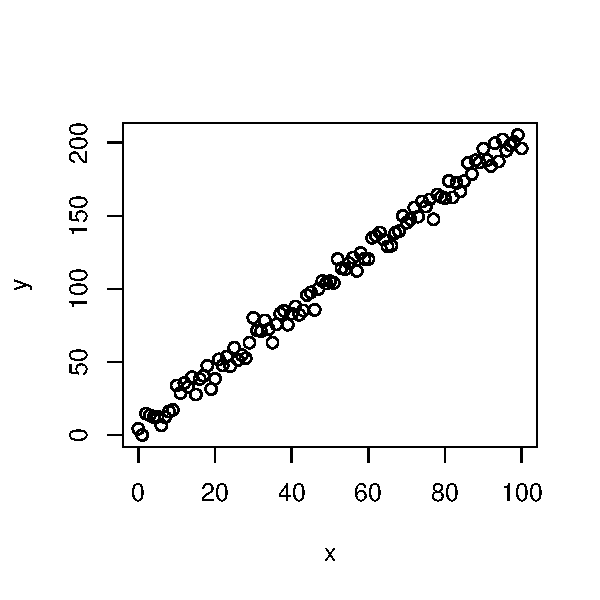
\includegraphics[width=85mm,height=85mm]{Manu_article_files/figure-latex/Figure-1-1} 

}

\caption{Figure caption}\label{fig:Figure-1}
\end{figure}

\end{document}
